\thispagestyle{myheadings}
\chapter{評価実験}

 収集した心拍データの心拍数上昇箇所の抽出処理が適切なのか,また表示したエフェクトが視聴者にはどのように感じるのかを評価するため実験を行う.
まずエフェクト重畳前の映画を視聴してもらった.安静にした状態で腕にスマートウォッチを取り付け,
映画を見る1分前から心拍数の取得を始め映画が終わるまでを計測した.環境は自宅でも気軽に臨場感が味わえることが目的なので,
普段映画を自宅で視聴する時と同じ環境で視聴した.次にエフェクトを重畳した映画も視聴してもらい,視聴後のアンケートも行った.

\section{心拍データの心拍数上昇箇所の抽出処理について}
 本節では心拍データの心拍数上昇箇所の抽出処理が適切に処理できていたか評価し考察する.

\subsection{心拍数上昇箇所の抽出方法についての評価}
 データを処理する際の閾値や設定が正確に処理できていたか評価する.
実験として3 本の映画に対し各3人のデータを収集した.映画は 007/ノー・タイム・トゥ・ダイ,キングコング/髑髏島の巨神,嘘喰いの 3 本にした.
映画は心拍数の変化が大きくなると仮定したアクション映画にした.集めたデータを処理した結果,
盛り上がりのシーンで心拍数が上昇している部分が抜き出せているものもあった.
また,エフェクトを表示する時間 from から to も閾値を超えた瞬間から下がるまでを記録できていた.
しかし人によっては心拍数が常に一定の人や変化が 激しい人などさまざまなためその全てに対応ができていなかった.
人によっては上昇箇所がたくさんあり,盛り上がりのシーン以外でも反応してしまった.
また心拍数の変化が少ない人では全く心拍数の上昇箇所を抜き出すことができなかった.
 心拍数が上昇している箇所をうまく抜き出せていない映画では,
抽出処理した心拍データを1つのJSONデータにまとめる際に混ざってしまいうまく抜き出せている心拍データだけを反映するのができていなかった.

\begin{figure}[H]
    \centering
    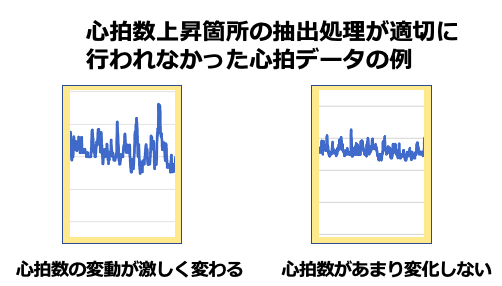
\includegraphics[width=13cm]{images/chapter4/miss.png}
    \caption{心拍数上昇箇所の抽出処理をした結果}
\end{figure}


\subsection{心拍数上昇箇所の抽出方法についての考察}
 心拍数が上昇している箇所を適切に抜き出せていない原因として,
始めの一分間を安静時の心拍数として決定するためその後の変化に対応できないからだと推測する.
はじめの1分間を安静時の心拍数として決定すると,
映画が進むにつれ徐々に心拍数が上がっていく人や逆に下がっていく人など閾値の設定が反映されなくなってしまったからだと考える.
また図のように映画を見る前の状態では落ち着いた心拍数で安定しているが,
映画を見始めると心拍数が安定していても興奮しているため平均心拍数が安静時よりも高くなっているからである.
 最終的に一つのJSONデータにまとめる際に盛り上がりのシーン以外も使いされてしまう課題について,
処理したそれぞれの心拍データを一つのJSONデータに追加していくだけなので,
姿勢を変えたなどのノイズもエフェクト表示に使われてしまった.対策として様々な心拍数の変化に対応するため,
平均を常に更新しそれに応じて閾値も変動させ,データを一つにまとめる際には複数人が反応を示している箇所だけを抜き出しまとめれば解決すると考える. 

\begin{figure}[H]
    \centering
    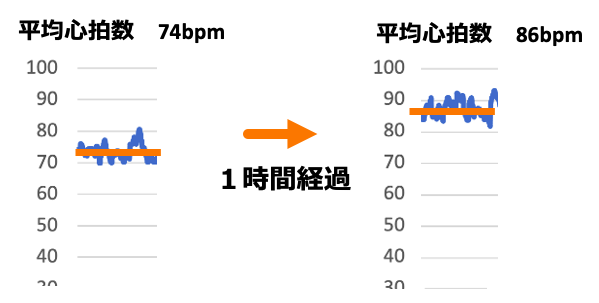
\includegraphics[width=13cm]{images/chapter4/bpmave.png}
    \caption{心拍数上昇箇所の抽出処理をした結果}
\end{figure}

\section{重畳提示の手法}
エフェクト選択後の視聴画面に対し10人のデータを収集し,評価方法としてエフェクト制作の目的を5段階評価でどれほど感じたかで集めた.
データを処理した結果として,Actionのエフェクトではキングコングを視聴し5の評価6件4の評価を6件と恐怖感や緊迫感を感じた意見があった.しかしエフェクトの色が赤色のみに固定されている,エフェクトが急に激しくなる意見に対応ができていなかった.改善策としてエフェクトの色を選択できるように変更し,エフェクト表示が変わる時にフェードアウトを追加する.AnimeのエフェクトではSPY×FAMILYを試聴し5の評価3件4の評価6件3の評価1件と面白さを与えるのが低かった.エフェクトの線が多く邪魔になった.アニメの中でもSFやコメディーなどに合わない意見に対応ができていなかった.改善策として効果線の太さを細くし変更,アニメのジャンルの中でもエフェクト選択画面を追加する.Horrorのエフェクトでは嘘喰いを視聴し4の評価2件4の評価6件3の評価2件と恐怖を軽減するのが低かった.画面全体が急に見づらくなった.恐怖を軽減するのに対応ができていなかった.改善策としてエフェクトのぼかしの不透明度を上げ,ぼかす範囲を狭める.

